\begin{wrapfigure}{r}{0.25\textwidth}
\begin{center}
%\framebox[4.0in]{$\;$}
%\fbox{\rule[-.5cm]{0cm}{4cm} \rule[-.5cm]{4cm}{0cm}}
 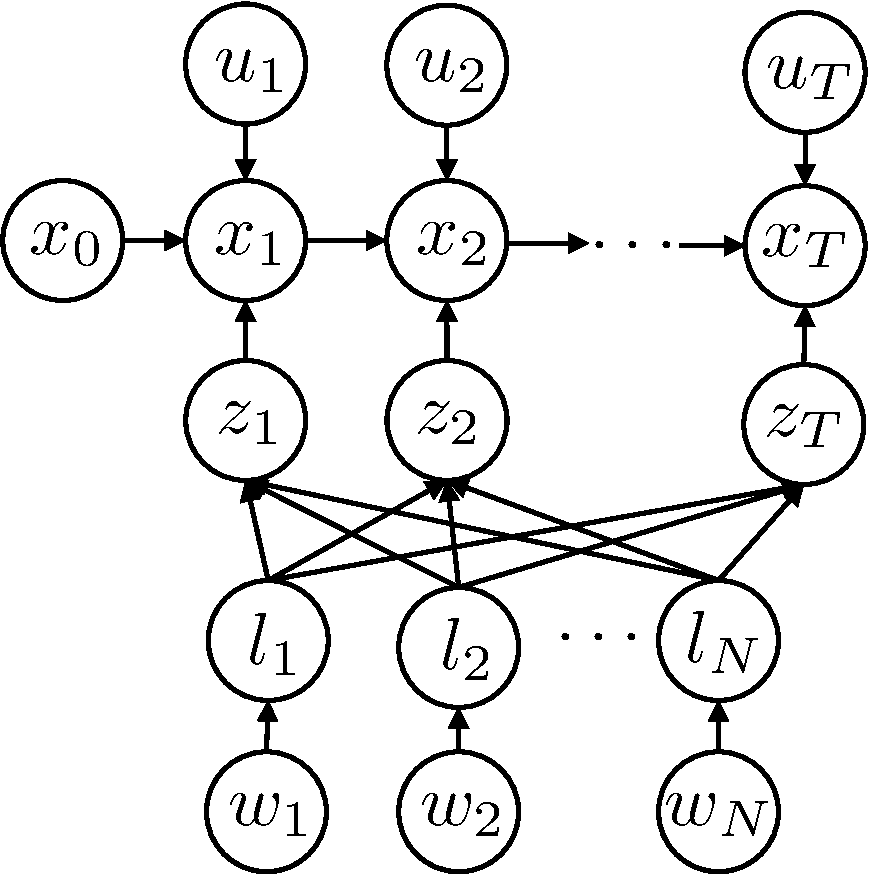
\includegraphics[width=0.22\textwidth]{fig/model} 
\end{center}
\caption{Graphical Model Formulation}
\label{fig:model}
\end{wrapfigure}

\section{Graphical Model Formulation}
Following \cite{isam} we formulate the SLAM problem in graphical models in Figure \ref{fig:model}. Specifically, the robot states are denoted by $X = \{x_i\}$ with $i \in 0, \dots T$, the landmarks by $L = \{l_j\}$ with $j \in 1,\dots, N$, the control inputs by $U = \{u_i\}$ for $i \in 1,\dots, T$ and the landmard measurements by $Z = \{z_k\}$ with $k \in 1, \dots, K$. In addition to the traditional SLAM formulation, we also add latent parameters $W = \{w_j\}$ with $j \in 1, \dots, N$  The joint probability of all variables and measurements are given by
\begin{equation}
P(X, L, U, Z, W) = \prod\limits_{i}P(x_i|x_{i-1}, u_i)\prod\limits_{k}P(z_k|x_{i_k}, l_{j_k}, w_k)
\label{eq:jointProb}
\end{equation}


Using a Gaussian representation for the sensor model, the process model and measurement equation follows
\begin{equation}
\begin{aligned}
x_i &= f_i(x_{i-1}, u_i) + w_i \\
z_k &= h_k(x_{i_k}, l_{j_k}) + v_k
\end{aligned}
\end{equation}
where $w_i$ and $v_k$ follow zero-mean normal distribution with covariance matrices $\Gamma_i$ and $\Sigma_k$. With this formulation, the second part of the equation \ref{eq:jointProb} is
\begin{equation}
P(z_k|x_{i_k}, l_{j_k}, w_k)\propto \exp\{-w_k((z_k - h(x_{i_k}, l_{j_k})^T)\Sigma^{-1}(z_k - h(x_{i_k}, l_{j_k}))\}
\label{eq:sensor}
\end{equation}
$w_k$ is the likelihood that the measurement comes from static landmark. In our case, we need to infer what those values are and ideally the process could be online or folows an incremental fashion. Possible solutions could be
\begin{itemize}
\item Using visual cues to cluster the landmarks to ``moving''/``static''. Challenges mainly lies in whether the features we use is reliable or not in terms of this clustering task.
\item Instead of using an expensive EM algorithm in \cite{rogers2010slam}, we design particle filters to incrementally update parameter $w_k$, making the whole process online.
\end{itemize}



